\documentclass[10pt]{beamer}
\usepackage[utf8]{inputenc}

\usepackage{multirow,rotating}
\usepackage{xcolor}
\usepackage{hyperref}
\usepackage{tikz-cd}
\usepackage{array}
\usepackage{siunitx}
\usepackage{mathtools,nccmath}%
\usepackage{etoolbox, xparse} 
\usepackage{csquotes}
\usepackage{listings}
\usepackage{qtree}
\usepackage{multicol}
\usepackage{lmodern}

\usetheme{Pittsburgh}
\usecolortheme{dolphin}

% set colors
\definecolor{myNewColorA}{RGB}{158, 27,50}
\definecolor{myNewColorB}{RGB}{158, 27,50}
\definecolor{myNewColorC}{RGB}{130,138,143} %{158, 27,50} % {130,138,143}
\definecolor{darkgreen}{rgb}{0.0, 0.5, 0.0}
\setbeamercolor*{palette primary}{bg=myNewColorC}
\setbeamercolor*{palette secondary}{bg=myNewColorB, fg = white}
\setbeamercolor*{palette tertiary}{bg=myNewColorA, fg = white}
\setbeamercolor*{titlelike}{fg=myNewColorA}
\setbeamercolor*{title}{bg=myNewColorA, fg = white}
\setbeamercolor*{item}{fg=myNewColorA}
\setbeamercolor*{caption name}{fg=myNewColorA}
\usefonttheme{professionalfonts}
\usepackage{natbib}
% \bibliographystyle{binat}
%\usepackage{filecontents} % for inline .bib file
\usepackage{hyperref}

\usepackage[ddMMyyyy]{datetime} 
\usepackage[normalem]{ulem}
%------------------------------------------------------------
% \titlegraphic{\includegraphics[height=0.75cm]{ua_eng_logo.png}} 

% logo of my university


\titlegraphic{%

\includegraphics[width=2.0cm]{ul-logo.png}
}

\setbeamerfont{title}{size=\large}
\setbeamerfont{subtitle}{size=\small}
\setbeamerfont{author}{size=\small}
\setbeamerfont{date}{size=\footnotesize}
\setbeamerfont{institute}{size=\footnotesize}
\title[]{
Diachronic study of semantic analogies 
%for (a) given language(s) across different time periods 
}%title
\subtitle{ 
Software project, group 5
}%%subtitle
\author[UL]{Averie (Ho Zoen) SO, NGO Van Duy, Scott TANKARD, Mathilde AGUIAR
}%%authors

\date[\textcolor{white}{Our title}]
{
\today{}}

\institute[]{Universit\'e de Lorraine}
% \setbeamercovered{invisible}
% \setbeamercovered{%
%   again covered={\opaqueness<1->{15}}}

%------------------------------------------------------------
%This block of commands puts the table of contents at the 
%beginning of each section and highlights the current section:
%\AtBeginSection[]
%{
%  \begin{frame}
%    \frametitle{Contents}
%    \tableofcontents[currentsection]
%  \end{frame}
%}
\AtBeginSection[]{
  \begin{frame}
  \vfill
  \centering
  \begin{beamercolorbox}[sep=8pt,center,shadow=true,rounded=true]{title}
    \usebeamerfont{title}\insertsectionhead\par%
  \end{beamercolorbox}
  \vfill
  \end{frame}
}
% ------Contents below------
%------------------------------------------------------------

% \begin{filecontents}{\jobname.bib}
% \end{filecontents}

\begin{document}

%The next statement creates the title page.
\frame{\titlepage}
\begin{frame}
\frametitle{Outline}
\tableofcontents
\end{frame}


% consider removing it if it's too redundant
% \AtBeginSection[]
% {
%   \begin{frame}
%     \frametitle{Table of Contents}
%     \tableofcontents[currentsection]
%   \end{frame}
% }

%------------------------------------------------------------
\section{Introduction}
% this section assigned to: 
\begin{frame}{Introduction}
\begin{itemize}
\item
\textbf{Project goal:} 
A project related to the 5th proposed project on cross-lingual analogy. 
Instead of across related languages, we are interested in a diachronic study and determining the level of similarity of the same language (e.g. English) across different historical periods according to semantic analogies.
\end{itemize}
\end{frame}

\begin{frame}{What we did so far}
\begin{itemize}
    \item Browsing and choosing datasets 
    \item Running 3 different baselines 
    \item More literature review on temporal word embeddings and temporal word analogies
\end{itemize}
\end{frame}
% end{my suffering} (>.<)


\section{Datasets}

\begin{frame}{Potential datasets}
Our first choice for English: 
    \begin{itemize}
        \item DUKweb: Diachronic UK web 
        \begin{itemize}
            \item Compile resources from Internet Archive of contemporary British English from 1996 to 2013 (granularity: years)
            \item Contains co-occurrences matrices and word vectors for each year 
        \end{itemize}

Other datasets from various languages:
        \item Datasets constructed from the SemEval Task:
        \begin{itemize}
            \item RuSemShift (Rodiana and Kutuzov, 2021) for Russian
            \item Kronos-it (Basile, Semeraro, Caputo, 2019) for Italian
            \item DIACR-Ita (Basile et al., 2020) for Italian
            \item LSCDiscovery (Zamora-Reina, Bravo-Marquez, Schlechtweg, 2022) for Spanish
            \item ZhShfitEval (Chen, Chersoni, Huang, 2022) for Chinese Mandarin 
            \item NorDiaChange (Kutuzov et al., 2022) for Norwegian
        \end{itemize}
    \end{itemize}
\end{frame}



\section{Literature review}
% this section assigned to: Mathilde
\begin{frame}{Szymanski, 2017}
    \onslide<1->{Temporal Word Analogies (TWA)} \\ 
    \textit{"A temporal word embedding is a pair of words which occupy a similar semantic space at different points in time."} \cite{szymanski2017temporal} \\
    Method used for discovering TWA : 
    
    \begin{enumerate}
        \item \textbf{Train independent Vector Space Models}: 1 VSM = 1 period of time. Uses Word2Vec to obtain the models.   
        \item \textbf{Transform all those VSMs into a unique common space}: Align different VSMs from the different periods. 3 methods are available : 
            \begin{itemize}
                \item \textbf{Non-random initialization}
                \item \textbf{Local linear regression} 
                \item \textbf{Orthogonal procrustes}
            \end{itemize}
        \item  \textbf{Compare a word's vector from different VSMs}: To define patterns of change over time. 
    \end{enumerate}
\end{frame}

\section{Baseline Work}

\begin{frame}{Szymanski et al. 2017 (TWAPY)}
    \begin{itemize}
        \item 1987 : reagan :: 1997 : clinton (US presidency)
        \item 1987 : mitterrand :: 1997 : mr\_chirac (French presidency)
        \item 1987 : gorbachev :: 1997 : mr\_yeltsin (From Soviet to Russian presidency)
        \item 1987 : soviet :: 1997 : russian (Historical event based on entities)
        \item 1987 : gemayel :: 1997 : denktash (Lebanese presidency, Hrawi \sout{denktash}) %(Imprecision by low resource?)
        \item 1987 : icbm :: 1997 : warheads (Strategic changes in modern warfare?)
        \item 1987 : philippines :: 1997 : united\_states (Political crisis)
        \item 1987 : internet :: 1997 : ... (OOV)
    \end{itemize}   

\end{frame}

\begin{frame}{Arefyev and Zhikov 2020 (BOS AggloSil)}
\begin{itemize}
    \item 
N Arefyev, V Zhikov. BOS at SemEval-2020 Task 1: Word Sense Induction via Lexical Substitution for Lexical Semantic Change Detection. In Proceedings of the Fourteenth Workshop on Semantic Evaluation, 171-179.
Bib: \cite{arefyev-zhikov-2020-bos}
Links:
\href{https://aclanthology.org/2020.semeval-1.20/}{web},
\href{https://aclanthology.org/2020.semeval-1.20.pdf}{pdf}

% https://www.ims.uni-stuttgart.de/en/research/resources/corpora/sem-eval-ulscd-eng

    \item
    Their main repo: 
    \url{https://github.com/DeadBread/BOS_AggloSil}
    
    \item
    Corresponding visualization tool (web app): 
    \url{https://github.com/DeadBread/SCD_WSI_tool/}

    \item BOS+AggloSil+DC:
    \enquote{%
    %For a particular target word its occurrences in old and new corpora are collected, and lexical substitutes are generated for each of them.
    WSI [word sense induction] is performed by clustering bag-of substitutes (BOS) vectors with agglomerative clustering employing silhouette score to select the number of clusters (AggloSil).
    Finally, we search for a decision cluster (DC), i.e. a cluster that has large number of occurrences from one corpus and small from another, and predict semantic change if such cluster exists.}
\end{itemize}
\end{frame}

\begin{frame}{BOS AggloSil contd.}
    \begin{itemize}
        \item Goal: Get the codebase working, before trying to decide to adapt it for our purposes or not
        
        \item We were able to familiarize ourselves with the codebase and run their example commands. 
    Challenges included: 
    \begin{itemize}
        \item codebase is old, and requires specific versioning (resolved by testing different python versions, creating a requirements.txt and conda environment with each problem ironed out);
        \item codebase is also not well documented (explored the code with various tools, including creating call graph diagrams with code2flow);
        \item not having enough RAM to run the code (resolved with teamwork, Averie was able to run it).
        \end{itemize}
        
    \end{itemize}
\end{frame}

\begin{frame}{Rosin et al., 2017}
    \begin{itemize}
        \item uses \textit{entity-relation} pairs to look for change in semantic \textit{relatedness} rather than \textit{similarity}
    \end{itemize}
    \begin{minipage}{.60\textwidth}
    \begin{itemize}
        \begin{itemize}
            \item \textit{‘in which time period were the words Obama and president maximally related?’}
            \item Obama-president vs. Obama-Trump
            \item relies on an additional relational corpus (YAGO2)
        \end{itemize}
    \end{itemize}
    \end{minipage}
        \begin{minipage}{.30\textwidth}
        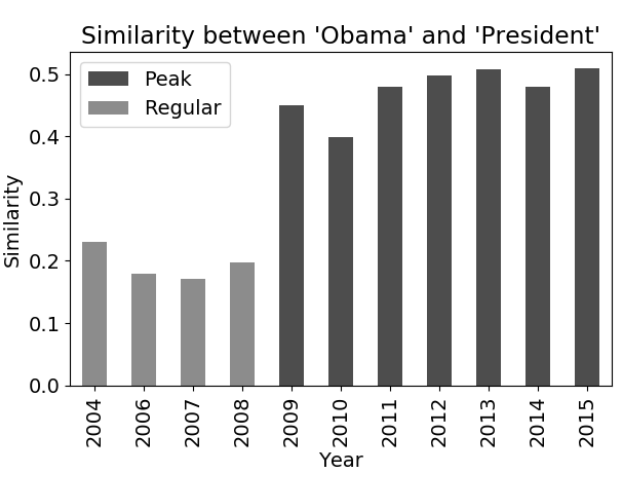
\includegraphics[width=4cm]{rosin_results.png}
    \end{minipage} 
    \begin{itemize}
        \item issues:
        \begin{itemize}
            \item available relations are rather limited, so we decided it won't be the main component of our project
            \item the purpose is more about temporal querying (factual) rather than exploring the semantics of words 
            \item haven't been able to run it yet due to missing NYT dataset
        \end{itemize}
    \end{itemize}   
\end{frame}


\section{Conclusion}
% this section assigned to: 
\begin{frame}{Conclusions and next steps}
\begin{itemize}
    
    \item Summary
    \begin{itemize}
        \item we decide to use domain-general, longitudinal ($\sim$ 1 century+ wide) datasets for multiple languages
        \item we would like to build on the codebase from Szymanski et al (2017) since it is the most similar for our purpose
        \item we explored alternative ways to use analogies (semantic relations) and to obtain semantic representations (BOS AggloSil)
    \end{itemize}

    \item Next steps
    \begin{itemize}
        \item since a lot of the literature and the codebase are kind of old (-2017), we plan to consult the SemEval shared task (2020) to experiment with various technical aspects to improve the results (how to generate embeddings, how to compare vector representations across time periods..)
        \item adapt the codebase to our datasets
    \end{itemize}
    
    \item Remaining questions
    \begin{itemize}
        \item understanding the (dis)advantages of using pretrained embeddings vs raw text datasets
    \end{itemize}
\end{itemize}
\end{frame}

\begin{frame}{Timeline}
\begin{itemize}
    
    \item Next two weeks (-18/11): focus on Twapy and get a working prototype using it (OR determine that it is not suitable). Determine what extra components/features we plan to add.

    \item December: Try to expand to other datasets

    \item January: polish the codebase, do testing.
\end{itemize}
\end{frame}


\section*{Resources}  
\begin{frame}[allowframebreaks]
        \frametitle{References}
        \bibliographystyle{amsalpha}
        %\bibliographystyle{plainnat}
        \bibliography{main.bib}
\end{frame}

\section*{Acknowledgements}  
\begin{frame}
    \textcolor{myNewColorA}{\huge{\centerline{Thank you!}}}
    \vspace*{0.5cm}

\textcolor{myNewColorA}{\Large{\centerline{Question time}}}

\end{frame}


\end{document}

%Rochester